\chapter{Specification for the Design}\label{specifiation}
In the feasibility study a set of specifications were obtained using behavioural modeling. In this chapter a small discussion of the results will be presented with additional specifications needed to implement the circuit design.

The specifications can be divided into two categories as listed below. 

$\bullet$ \textbf{Requirements for the integrators}: The requirement for the total noise was derived in the feasibility study to find the optimal size for the capacitors used by the integrators and the summing node. In the feasibility study it was found out that matching requirements were needed, and with parameters given by \textit{Microchip} \cite{private}, we could calculate realizable capacitors values. In this thesis the matching requirements are the same, but the parameters are different, thus giving us a new set of capacitors values. The switch's on resistance were found after an exhaustive iteration of simulation.

$\bullet$ \textbf{Requirements for the Amplifier}: After an exhaustive iteration of simulation, the specifications for the finite DC gain, GBW and slew rate were found. The output-swing and the load capacitance seen from each output of the OTAs is also presented here. 

\section{Sizing of Capacitors}
The proposed architecture was a discrete-time third-order single-bit single-loop feedforward $\Delta\Sigma$ modulator, as shown in figure \ref{fig:input}. The transfer function for the non-inverting integrators is given by,

\begin{equation}\label{transfer_integrator}
    H(z) = \frac{C_s}{C_i}\cdot \frac{z^{-1}}{1 - z^{-1}}
\end{equation}

where $C_s$ is the sampling capacitor and $C_i$ is the integrating capacitor. The coefficients $b_1, c_1$ and $c_2$ describe the relationship between these capacitors for integrator 1, 2 and 3 respectively. For instance the capacitors' relationship in integrator 1 can be described by

\begin{equation}
    b_1 = \frac{C_s}{C_i}
\end{equation}

The feedforward coefficients $a_1, a_2$ and $a_3$ describe the parallel network of capacitors in the summation circuit shown in appendix ??

The coefficients found in the feasibility study are given in table \ref{scale}.

\begin{table}[h]
\centering
\caption{Coefficients}
\label{scale}
\begin{tabular}{|l|l|l|}
\hline
Coefficients  &      \\ \hline
$b_1$         & 0.32 \\ \hline
$c_2$         & 0.69 \\ \hline
$c_3$         & 0.16 \\ \hline
$a_1$         & 2.56 \\ \hline
$a_2$         & 1.32 \\ \hline
$a_3$         & 1.27 \\ \hline
\end{tabular}
\end{table}

The matching requirements is given in table \ref{match}.

\begin{table}[h!]
\centering
\caption{Matching requirement}
\label{match}
\begin{tabular}{|l|l|}
\hline
Coefficients & Matching \\ \hline
$a_1$           & $\pm4\%$        \\ \hline
$a_2$           & $\pm4\%$        \\ \hline
$a_3$           & $\pm4\%$        \\ \hline
$c_2$           & $\pm2\%$      \\ \hline
$c_3$           & $\pm1\%$        \\ \hline
\end{tabular}
\end{table}

Using the coefficients with the matching requirements and parameters given by \textit{Microchip}, the final values can be computed. The capacitors that realize  $a_1, a_2$ and $a_3$ are matched to the same reference (the feed-forward capacitor). Thus, the following realization of the coefficients is proposed:

\begin{table}[h!]
\centering
\caption{Realizable coefficients}
\label{RC}
\begin{tabular}{|l|l|l|l|}
\hline
Coefficients & Ideal value & Fractional value & Cap realization \\ \hline
b1           & 0.32        & 542/1779         & 2.05p/6.58p     \\ \hline
a1           & 2.56        & 64/25            & 236.8fF/92.5fF \\ \hline
a2           & 1.32        & 33/25            & 122.1fF/92.5fF  \\ \hline
a3           & 1.27        & 32/25            & 118.4fF/92.5fF  \\ \hline
c2           & 0.69        & 7/10             & 76fF/106.4fF \\ \hline
c3           & 0.16        & 3/19             & 45.6fF/288.8fF   \\ \hline
\end{tabular}
\end{table}

\section{Switches' on-resistance}\label{on-resistance}
The size of the switches' on-resistance have to be specified to estimate the cost of implementing it on transistor-level. Having small on-resistance will lead to bigger area usage, and it will therefore be costly to implement. The goal in the feasibility study was to find the largest on-resistance for the integrators that will give the desired performance. The final values are summarized in table  

\begin{table}[H]
\centering
\caption{Final specification for the switches' on-resistance}
\label{spec_res}
\begin{tabular}{|l|l|l|l|l|l|}
\hline
Specifications & Integrator 1 & Integrator 2 & Integrator 3 & Summing node &    \\ \hline
Ron            & 0.9            & 1.5          & 1.6          & 1.7          & $k\Omega$ \\ \hline
\end{tabular}
\end{table}

\section{Finite DC-gain}

Finite DC-gain will give integrator leakage, which can in general be expressed as:

\begin{equation}
    H(z) = \frac{1}{z - \alpha}, \alpha = 1 - \frac{1}{A_0}
\end{equation}

This means the integrator has a DC-gain limited by opamp's open-loop gain, which again means that the DC-attenuation of the NTF is also limited. In general the cascade of opamps' gains much be much higher than the desired NTF DC-attenuation, or in other words higher than the resolution. The effect of limiting gain is shown in figure \ref{fig:DC_gain_spec}. AS seen the third order modulator has small open-loop gain, raging from 35dB to 45dB. The reason being all the NTF's zeroes will be in DC. Therefore the cascade of open-loop gains of the integrators are sufficient enough to give the desirable performance. Another advantage of having small gains is that the specifications for gain for each OTA are relaxed, thus one can easily achieve the requirement with a one stage OTA. 

\begin{figure}[H]
\centering
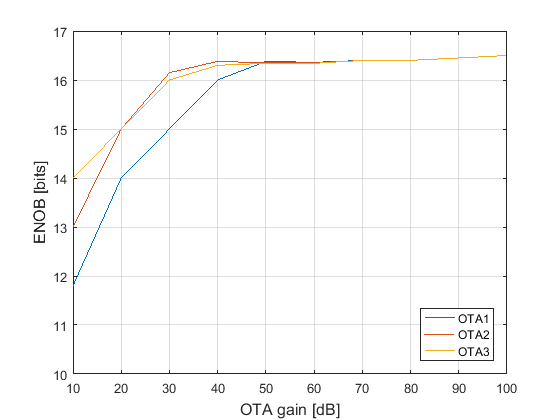
\includegraphics[scale=0.7]{images/DC_gain_spec.png}
\caption{ENOB limitation due to finite open}
\label{fig:DC_gain_spec}
\end{figure}

\section{Output swing}\label{out_put_swing}
In figure \ref{fig:output_swing} we see the output swing of integrator 1, 2 and 3. We have that for integrator 1 and 2 the output swings from 0.6 to 1.2, while for integrator 3 it swings from 0.7 to 1. This gives us voltage change ($\Delta V_{1,2}$) of 0.6 for integrator 1 and 2, and $\Delta V_3$ of 0.3 for integrator 3. It is worth mentioning that when the output voltage is closer to limits, the response is distorted.    

\begin{figure}[h]
\centering
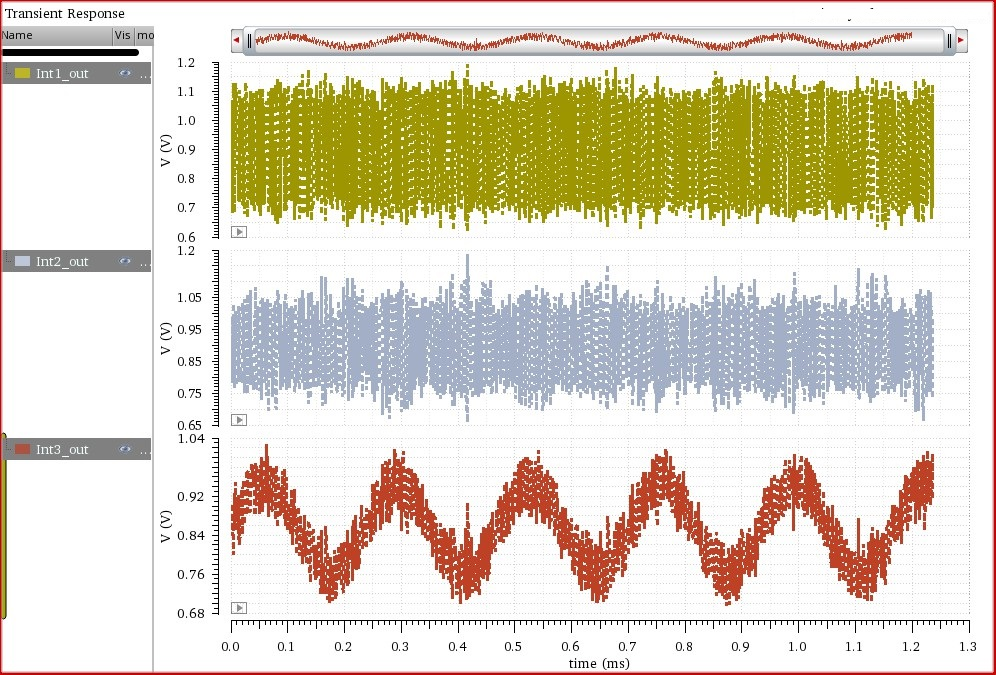
\includegraphics[scale=0.45]{images/output_swing.jpg}
\caption{Output swing of integrator 1, 2 and 3}
\label{fig:output_swing}
\end{figure}

\section{Gain-Bandwidth Product an Slew-Rate}

Finite gain-bandwidth (GBW) of the OTA will lead to incomplete linear settling as the output will not settle to its final value. This will cause the ENOB to degrade, therefore we need to find sufficient GBW to achieve the desired ENOB. The degradation of ENOB with falling GBW is shown in figure \ref{fig:GBW_spec}. It was found out the minimal GBW should be between 28MHz and 38MHz. If we choose smaller GBW, the performance will degrade rapidly. Making this specification one of the most critical.

\begin{figure}[h]
\centering
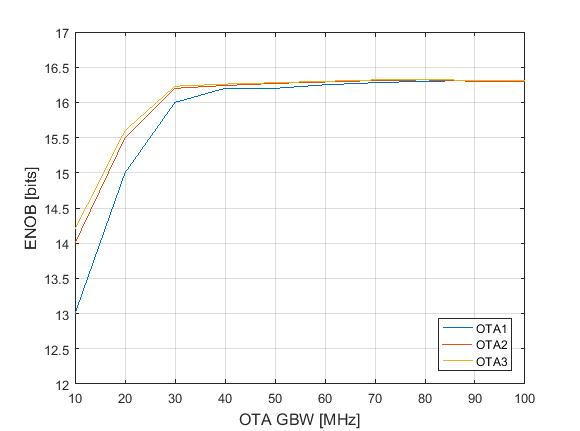
\includegraphics[scale=0.55]{images/GBW_spec.jpg}
\caption{ENOB limitation due to GBW}
\label{fig:GBW_spec}
\end{figure}

Unlike linear settling error, slewing causes non-linear settling error which degrade the ADCs linearity. The slew- rate must be high enough to avoid slewing to cause non-linear settling error. Meaning it must be high enough to settle the output in $\frac{T_s}{2}$, where $T_s$ is the sampling period. This gives us the requirement for minimum slew-rate:

\begin{equation}\label{sr}
    \frac{\Delta V}{SR} > \frac{T_s}{2}
\end{equation}

where $\Delta v$ is the output change in the integrator. We from section \ref{out_put_swing}, that the output change is 0.6 for integrator 1,2 and 0.3 for integrator 3. By performing transient analysis we found out the slew-rates given by equation \ref{sr} are not sufficient. The calculated and the final simulated values are summarized in table \ref{SR_final}.

\begin{table}[H]
\centering
\caption{Theoretical and Simulated Values of SR}
\label{SR_final}
\begin{tabular}{|l|l|l|}
\hline
Integrator & Calculated & Simulated \\ \hline
1           & 12MV/sec   & 28MV/sec  \\ \hline
2           & 12MV/sec   & 28MV/sec  \\ \hline
3           & 6MV/sec    & 28MV/sec  \\ \hline
\end{tabular}
\end{table}

\section{Load Capacitance}
To be able to design the OTAs correctly so that they function properly in the whole system, we need to find the load capacitance they see at their output. Using method introduced in \cite{load}, we can estimate what the load capacitance for each OTA will be. As an example we can compute for the first OTA. We have that.

\begin{equation}\label{cap_load}
    C_{L1} = C_{s1}||C_{i1} + C_{s2} + C_{ff1} + 0.2\dot(C_{i1} + C_{s2} + C_{ff1}) \approx 3.5p 
\end{equation}

where $C_{s1}$, $C_{i1}$ and $C_{ff1}$ are the sampling, integrating and feedforward capacitor of the first integrator. Same way we can find the load capacitance for second and third OTA, and they are $0.6p$ and $0.3p$ respectively. 

\section{Specifications of the Amplifier}
Table \ref{spec_ota} summarize the requirements for the amplifiers of integrator 1, 2 and 3. It has also been included a specification for phase margin. It has been chosen to be greater than $60^\circ$, because it allows for the fastest settling time when attempting to follow a voltage step input \cite{phase}. 

\begin{table}[H]
\centering
\caption{Specifications of the Amplifiers}
\label{spec_ota}
\begin{tabular}{|l|l|l|l|}
\hline
Parameter        & OTA1     & OTA2     & OTA3     \\ \hline
$A_O$             & $>$45dB     & $>$35dB     & $>$35dB     \\ \hline
GBW              & $>$38MHz    & $>$30MHz    & $>$28MHz    \\ \hline
SR               & $>$28MV/sec & $>$28MV/sec & $>$28MV/sec \\ \hline
Output Swing     & 0.6$<$Vout1$<$1.2 & 0.6$<$Vout2$<$1.2  & 0.7$<$Vout3$<$1         \\ \hline
Phase Margin     & $>$60$^\circ$       & $>$60$^\circ$       & $>$60$^\circ$       \\ \hline
Load Capacitance & 3.5p     & 0.6p     & 0.3p     \\ \hline
\end{tabular}
\end{table}

\section{Impact of nonidealities}

The non-ideal model of the modulator was simulated using the first three specifications given by table \ref{spec_ota}, and the capacitance summarized in table \ref{RC}. The output spectra is shown in figure \ref{fig:psd_non_ideal}, where the SNR and ENOB values are also shown. It can be noted that the main objective of achieving ENOB of 16 bits is satisfied.   

\begin{figure}[ht]
\centering
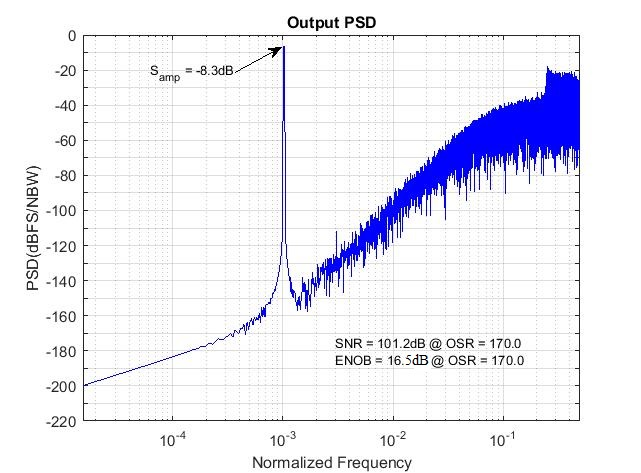
\includegraphics[scale=0.55]{images/psd_out_spec.jpg}
\caption{PSD of the output signal using non-ideal model}
\label{fig:psd_non_ideal}
\end{figure}
